\chapter{Projektbeskrivelse}

\section{Projektgennemførelse}
Projektet startede med, at der blev lavet en tidsplan, hvor der var mulighed for ændringer undervejs, dog var der nogle faste deadlines, som skulle følges. De forskellige deadlines ledte op til, at man kunne arbejde efter vandfaldsmodellen, da projektet startede med, at der blev lavet kravspecifikation og accepttest, som beskrev de krav, som programmet skulle kunne udfylde. Derefter var næste deadline, at der skulle laves design, ligesom viste forskellige diagrammer over, hvordan programmet skulle opbygges og hvad der skulle indeholde. Derefter blev programmeret færdiggjort og testet og til sidst finpudset. \\ \\
Altså er der i dette projekt blevet arbejdet efter vandfaldsmodellen, som benyttes, når man arbejder med software, ligesom der er blevet gjort i det pågældende projekt. Vandfaldsmodellen er opbygget på sådan en måde, at man arbejder med de forskellige dele som et vandfald, hvor man tager en af del af gangen og bevæger sig ned gennem de forskellige. De forskellige deadlines vi har haft stemmeroverens med de forskellige led i vandfaldsmodellen, som ses i figur(NUMMER)

\begin{figure}[H]
	\centering
	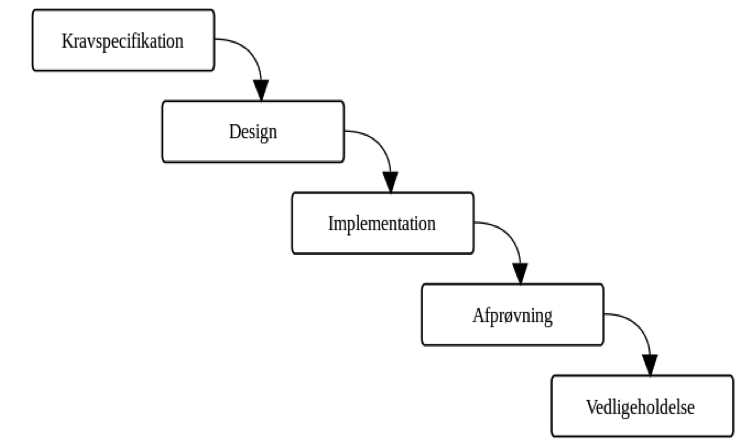
\includegraphics[width=1\textwidth]{Figurer/Snip20150522_15}
	\caption{Vandfaldsmodel}
\end{figure}

Projektgruppen har været på 8 medlemmer, som er blevet delt ind i 2 grupper, således at arbejdsbyrden blev delt. Den ene gruppe arbejdede med softwareudviklingen, mens den anden gruppe arbejdede med dokumentation og udarbejdelsen af design. Da gruppen har været opdelt, har der været projektmøde hver uge, hvor gruppen har opdateret hinanden og rettet tidsplanen til, hvis det var nødvendigt.


\section{Metode} 
Dette afsnit har til formål, at beskrive hvilke metoder der er benyttet i udarbejdelsen af dette projekt. Primært er der tale om metoder fra faget ISE, samt Sundhedsvidenskab.\\ 
Desuden bliver der i dette afsnit også beskrevet hvilken arbejdsredskaber der er benyttet til udførelse af projekt, rapport og dokumentering.\\ \\
Til beskrivelse, samt opbygning er EKG-målings systemet, er der fra ISE benyttet metoden SysML. SysML er en metode der vha. digrammer analyserer, specificerer, designer og verificerer et givet system. Altså er metoden benyttet til at beskrive systemets opbygning og kommunikationen. Systemets virkning og de hvordan de enkelte dele interagerer er beskrevet ved SD, som er specefik for hver enkelt use case.\\ 
Yderligere er der en applikationsmodel, hvor et samlet overblik over systemet er beskrevet. Denne model består af en domænemodel, hvor alle aktiviteterne i systemet er beskrevet, samt en tilhørende klasse applikationsmodel. Desuden er SD også benyttet til at lave metoderne i applikationsmodellen.\\ 
Softwaren er beskrevet gennem metoden UML, helt specifikt ved et UML klassediagram. Klassediagrammet viser hvilke klasser og metoder al softwaren (med undtagelse af blackbox) består af, samt hvordan systemet er bygget op efter trelagsmodellen.\\
Baggrundsafsnittet, afsnit 3, er udarbejdet ved tekstanalyse og kildekritik, ud fra sundhedsvidenskabelige bøger og IT teori.\\ \\
Af benyttede arbejdsredskaber, er der først og fremmest brugt en fælles arbejdsplatform, GitHub. GitHub er en online platform, hvor der er mulighed for at foretage ændringer samtidigt, og gemme i en fælles mappe, yderlige er der mulighed for en detaljeret versionshistorik. Alle SysML- og UML-diagrammer er udarbejdet i programmet Visio. Koden er skrevet i sproget c\#, i programmet Visual Studio. Visual Studio spiller også sammen med programmet WaveForms generator, i forbindelse med simulering af EKG-signalet. Selve rapporten, mødereferater, logbog og dokumentationen er udformet i tekstprogrammet LaTex. Yderligere er Facebook brugt til mødeindkaldelse og generel kommunikation.



\section{Specifikation og analyse}
I udarbejdelsen af analysen var der mange komplikationer. Dette skyldes primært, at atrieflimren ikke nødvendigvis påvirker et EKG-signal på samme måde, hver gang.\\ \\
Først var der tiltænkt en analyse som skulle tage udgangspunkt i den originale definition for atrieflimren. Måden dette skulle foregå på, var at tage et gennemsnit af baseline, og derefter detektere hvor mange gange, der skete en svingning over baseline. Her skulle der så tjekkes, om svingningerne overtrådte en tærskel. Denne tærskel skulle vurderes ud fra den patofysiologiske baggrund for sygdommen. Efter visualisering af reelle målinger, blev denne metode dog afskrevet, da baseline ikke bliver repræsenteret ved en regulær linje i reelle signaler. \\ \\ 
Derefter blev der udtænkt en metode med en dynamisk baseline. Denne metode viste sig meget tideligt i udviklingsprocessen, til ikke at være kompatibel. Den største komplikation ved denne metode, er at finde en algoritme, kunne udelukke de kendte takker, som karakteriserer et EKG-signal. Hvis denne algoritme ikke blev fundet, ville den dynamiske baseline altid ligge et stykke over den reelle baseline, grundet de høje R-takker. \\ \\
De to første metoder blev aldrig færdiggjort, da problemerne opstod, efter pseudokode begyndte at blive udarbejdet. Herefter gik gruppen til vejleder for at finde en alternativ løsning til analysen. Vejleder fik herefter input fra en anden professionel, og kunne derefter hjælpe med at udarbejde en analyse, som virkede.\\ \\
Vejleder kunne oplyse at atrieflimren har specifikke kendetegn, hvis der bliver analyseret på EKG-signalets amplituder inden for specifikke frekvenser, og det er ud fra denne information, at den endelige analyse blev udarbejdet. 

\section{Arkitektur}
Softwaren er bygget op i henhold til trelagsmodellen, hvor GUI’erne fungerer som programmets brugerinterface, med et login-vindue, et CPR-vindue og et EKG-vindue. Her fungerer EKG-vinduet, som det primære vindue, hvor EKG-signaler kan måles. Grafiklaget er yderligere beskrevet i dokumentationen, men kan også visualiseres ud fra figur XX nedenfor.

\begin{figure}[H]
	\centering
	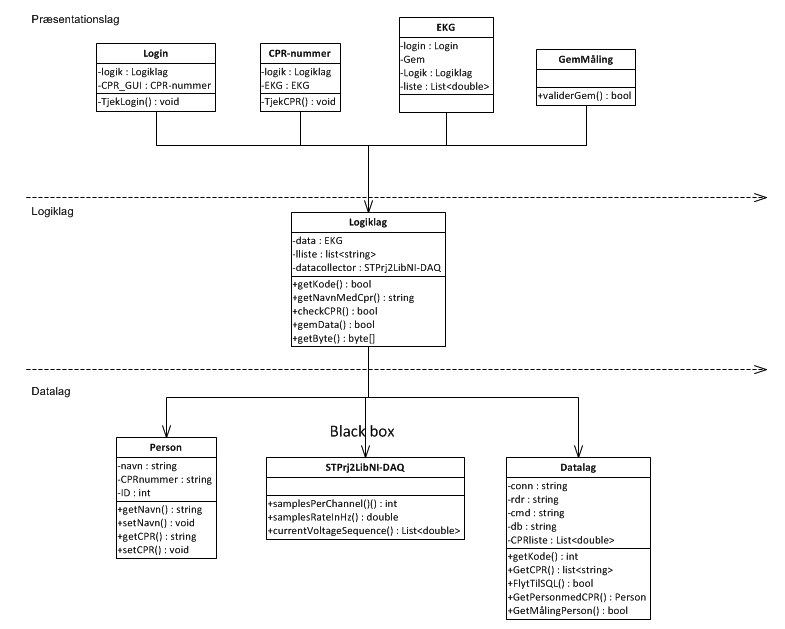
\includegraphics[width=1\textwidth]{Figurer/Snip20150512_9}
	\caption{UML-klassediagram}
\end{figure}
 
Logiklaget kan ses som kernen i softwaren. Det er her alt data bliver behandlet fra datalaget, samt videresender data fra målinger til datalaget. Det er blandt andet her analysen af målingen sker, og hvor indtastede oplysninger bliver valideret. Logiklaget fungerer som bindeleddet mellem de data, som kommer fra datalaget, og GUI’erne. \\ \\
Datalaget er til, for primært at håndtere forbindelsen med hardwaren og databaserne. I denne klasse bliver der skabt forbindelse til både SQL og DAQ. Datalaget henter data fra den private database, som logiklaget bruger til validering. Denne klasse gemmer også data givet fra logiklaget i både den private- og offentlige database. Klassen logiklag og datalag er beskrevet yderligere i dokumentationen. \\ \\
For at beskrive koden yderligere, er der lavet en domænemodel. Domænemodellen repræsenterer hele koden, altså hvordan flowet imellem klasserne går, og hvilken overordnet kommunikation, der foregår. Alle vinduerne repræsenterer GUI’er og alle tabeller er tabellerne i den private database. Domænemodellen kan ses på figur XX. 

\begin{figure}[H]
	\centering
	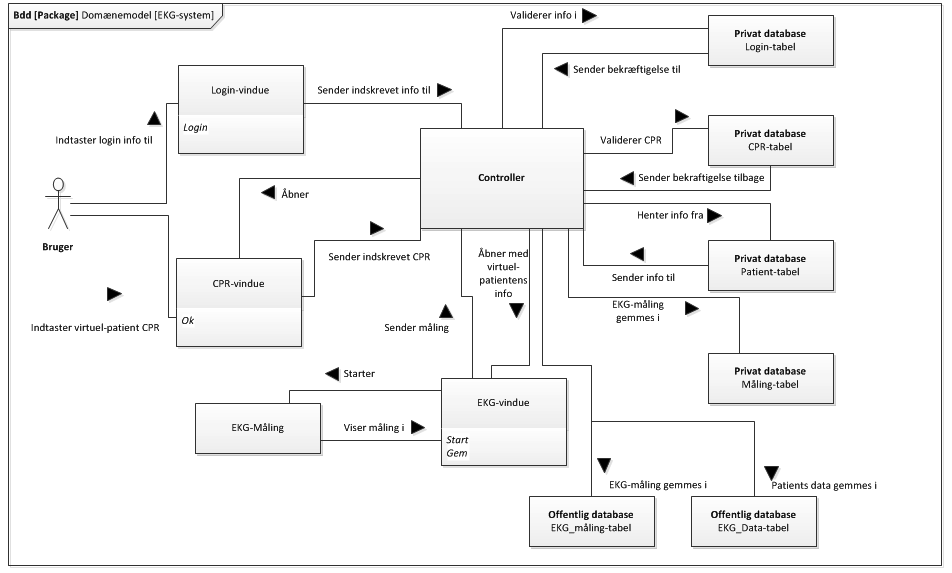
\includegraphics[width=1\textwidth]{Figurer/Snip20150525_18}
	\caption{Domænemodel}
\end{figure}


\subsection{Design}

\subsection{Implementering}

\subsection{Test}

\section{Resultater og diskussion}

\section{Opnået erfaringer}

\section{Fremtidigt arbejde}
Som følge af at projektet er tiltænkt som en prototype, er der løbende gennem projektudførelsen opstået en masse muligheder og idéer for videreudvikling af systemet. \\\\
Den første helt basale idé, som også er forsøgt udført sideløbende i projektet, er etablering af en "opret ny patient" funktion. Funktionen skal muliggøre, at den sundhedsprofessionelle kan oprette en ny patient i systemet, i forbindelse med indtastning af patientens CPR-nummer. Funktionen skal fungere således, at hvis ikke det indtastede CPR-nummer i forvejen er kendt i systemet, skal skridtet efter CPR-vinduet være et nyt "Opret Patient"-vindue. Her skal den sundhedsprofessionelle kunne indtaste relevante oplysninger omkring patienten, og til slut oprette patienten i både den private- og offentlige database.\\\\
Et ideelt område til videreudvikling er brugervenlighed, både på software plan og i særhed på hardware plan.\\
Software kun udvikles i en retning, hvor det bliver lettere og mere overskueligt for den sundhedsprofessionelle, at analysere og evaluere EKG-signalet. En forbedring ville være, at der skal være mulighed for at trække en eller flere x- og y-cursors ned over EKG-signalet, og dermed få vist amplitude og tid, og relevante intervaller. Herefter kunne en mulighed være, at de observerede værdier kunne gemmes som tilhørende tekst til det specifikke EKG-signal. \\
Sideløbende, imens EKG-målingen foretages, vil det være muligt, at have direkte adgang til den pågældende patients sygejournal. Adgangen til sygejournalen skal kunne læse i en et andet vindue, som er synligt samtidig med EKG-vinduet arbejder, hvorefter det er muligt at skifte mellem disse vinduer, og tilføje ændringer, notater etc. i journalen. Med andre ord skal systemet understøtte EPJ\\ \\
Den endelige udgave af softwaren skal implementeres på et mere brugervenligt interface, eksempelvis en tablet eller lignende. Samtidig skal systemet være tilknyttet en håndholdt EKG-måler, i form af en holter, hvorefter softwaren aflæser data fra, og udskriver på tabletten. Desuden skal det være muligt for den sundhedsprofessionelle at vælge indstillinger, alt efter hvad der ønskes analyseres for. Det endelige produkt er kun tilpasset analyse for atrieflimren, men det skal være muligt at kunne vælge, undersøgelse for eksempelvis andre sygdomme som ventrikelflimren, ST-elavation osv. De forskellige undersøgelser skal derudover også kunne mikses på kryds og tværs, hvis patienten har blandede symptomer, således at der søges for flere sygdomme. Dette vil medføre, at den sundhedsprofessionelle kan tage tage udstyr med sig på hjemmebesøg, såvel som at patienten selv kan foretage en måling.

